\documentclass[a4paper, 12pt]{article}

\usepackage{geometry}
\geometry{a4paper,
total={170mm,257mm},left=2cm,right=2cm,
top=1cm,bottom=2cm}
\usepackage{wrapfig}
\usepackage{graphicx}
\usepackage{mathtext}
\usepackage{amsmath}
\usepackage{siunitx} % Required for alignment
\usepackage{multirow}
\usepackage{gensymb}
\usepackage{rotating}
\sisetup{
  round-mode          = places, % Rounds numbers
  round-precision     = 2, % to 2 places
}

\usepackage[T1,T2A]{fontenc}

\usepackage[russian]{babel}

\graphicspath{{pictures/}}


\title{\begin{center}Лабораторная работа №2.2.1\end{center}
Исследование взаимной диффузии газов.}
\author{Каграманян Артемий, группа Б01-208}
\date{\today}

\begin{document}

\maketitle

\section{Аннотация}
\textbf{Цель работы:} Зарегистрировать зависимость концентрации гелия в воздухе от времени с помощью датчиков теплопроводности при разных начальных давлениях смеси газов и измерить коэффициент взаимной диффузии по результатам измерений. \\
\\
\textbf{Оборудование:} Измерительная установка (см. рис. ), форвакуумный насос, баллон с газом, манометр, источник питания, магазин сопротивлений, гальванометр, секундомер
\section{Теоритическая справка}
Диффузией называется самопроизвольное перемешивание молекул из-за их хаотичного теплового движения. В нашей системе давления во всех точках равны, так как иначе будет слишком сильное перемещение газов из одной точки в другую до того момента, пока не установится равенство. \\
Наша система состоит из двух сред, обозначим их за \(a \ и \ b\). Плотности потоков в этом случае будут равны:
\[j_{a} = -D_{ab}\frac{\partial n_a}{\partial x}, \ j_{a} = -D_{ba}\frac{\partial n_b}{\partial x},\]
где, \(D_{ab} = D_{ba} = D\) - коэффициент взаимной диффузии\\
В нашем случае концентрация воздуха намного больше, чем концентрация гелия (так как мы рассматриваем диффузию примеси гелия). Обозначим \(n_{He} \ за \ n\). Поэтому мы будем рассматривать только диффузию гелия на стационарном фоне воздуха. \\
\\
В нашей установке есть два сосуда объемами \(V_1 \ и \ V_2\), соединенные трубкой сечения \(S\) и длины \(l\). В начальный момент конуентрации гелия в этих сосудах не равны, но в конце диффузии они выравниваются. Сечение трубки много меньше размеров сосудов, поэтому можно говорить, что концентрация гелия в сосудах одинакова в любой точке, а процесс выравнивания концентраций осуществляется только благодарая диффузии в трубке.
\\
\\
Предположим, что процесс диффузии - достаточно медленный процесс, чтобы концентрация в сосудах изменялась линейно, и поток через трубку можно измерить по формуле (квазистационное приближение):
\[J = -DS\frac{n_1 - n_2}{l}\]
Найдем, как изменяются $n_1$ и $n_2$ от времени. По закону сохранения вещества: \[V_1 n_1 + V_2 n_2 = const \Rightarrow V_1 dn_1 = - V_2 dn_2 = Jdt = -DS\frac{n_1 - n_2}{l}dt\]
\[\frac{dn_1}{dt} = -DS\frac{n_1 - n_2}{lV_1}, \frac{dn_2}{dt} = DS\frac{n_1 - n_2}{lV_2}\]
\[\frac{dn_1}{dt} - \frac{dn_2}{dt} = -DS\frac{n_1 - n_2}{l}(\frac{1}{V_1} + \frac{1}{V_2})\]
Сделав замену $d(\Delta n) = d(n_1 - n_2)$ и проинтегрировав получившееся, получим следующее: \[\Delta n = \Delta n_0 e^{-\frac{t}{\tau}}, \ \tau = \frac{V_1V_2}{V_1 + V_2} \frac{l}{SD}\]
Для проверки квазистационного приближения нужно убедиться, что время характерной диффузии одно частицы много меньше, чем \(\tau\): \(t_д \sim \frac{l^2}{D} \ll \tau\).
\\
\\
Для измерения концентрации гелия в сосуде используются датчики теплопроводности смеси. Они работают следующим образом: В сосуде расположена проволока, по которой мы пускаем ток. Проволока нагревается, а смесь проводит тепло от проволоки к стенкам сосуда. Таким образом, тепло, которое передалось стенке за единицу времени, составляет:
\[Q = \kappa \frac{2\pi l}{ln(R_ц/r_{пр})}(T_1 - T_2),\]
где \(\kappa\) - теплопроводность смеси, \(L\) - длина проволоки, \(T_1 \ и \ T_2\) - температуры проволоки и стенки сосуда.
\\
Для измерения разности концентраций гелия в сосудах используется мостовая схема, в которой есть гальванометр. В нашей работе он показывал напряжениие на нем. При достаточно маленьких изменениях концентраций величина тока, проходящего через него, пропорциональна разности концентраций. В таком случае, показания гальвонометра:
\[N = N_0e^{-t/\tau}\]
Также следует отметить, что коэффициент диффузии можно оценить следующим образом:
\[D = \frac{1}{3}v_{тепл}\lambda, \  \lambda = \frac{1}{n_0\sigma},\]
где \(\lambda\) - длина свободного пробега частицы, \(n_0\) - концентрация фона, \(\sigma\) - эффективное сечение столкновений.
\newpage
\section{Экспериментальная установка}
\begin{figure}[h]
    \centering
    \includegraphics[width=0.6\linewidth]{2.2.6 pic.png}
    \caption{схема установки}
\end{figure}
Установка состоит из двух сосудов объемами \(V_1 \ и \  V_2\), в которых находятся датчики теплоемкости. Эти сосуды соединены с атмосферой, насосом и гелием с помощью стеклянных трубочек. Также здесь присутствует дозатор, который впускает в систему гелий определенными порциями. В момент, когда мы открываем \(K_3\) и начинается диффузия, на компьютере отмечаются показания гальванометра в виде графика.
\newpage
\section{Выполнение работы}
В начале каждого измерения нужно откалибровать мост под каждое рабочее давление. Для этого нужно запустить в сосуды воздух до требуемого рабочего давления, предварительно откачав перед этим систему, и подкрутить мост, чтобы вольтметр показывал примерно \(0 \ мВ\). Затем в один из сосудов впускаем гелий до давления \(0.2 \ P_{раб}\), а во второй сосуд -  воздух до давления \(1.635 \ P_{раб}\) (это при закрытом \(K_3\)). Далее мы отделяем от системы эти два сосуда и соединяем их между собой, ждем 15 секунд, чтобы в них установилось одинакове давление, открываем \(K_3\) и начинаем снимать показания вольтметра. \\
\\
Мы проведем 5 измерений для разных рабочих давлений, а именно для \(40, 60, 80, 100, 120 \ торр\). 

\begin{figure}[h]
    \centering
    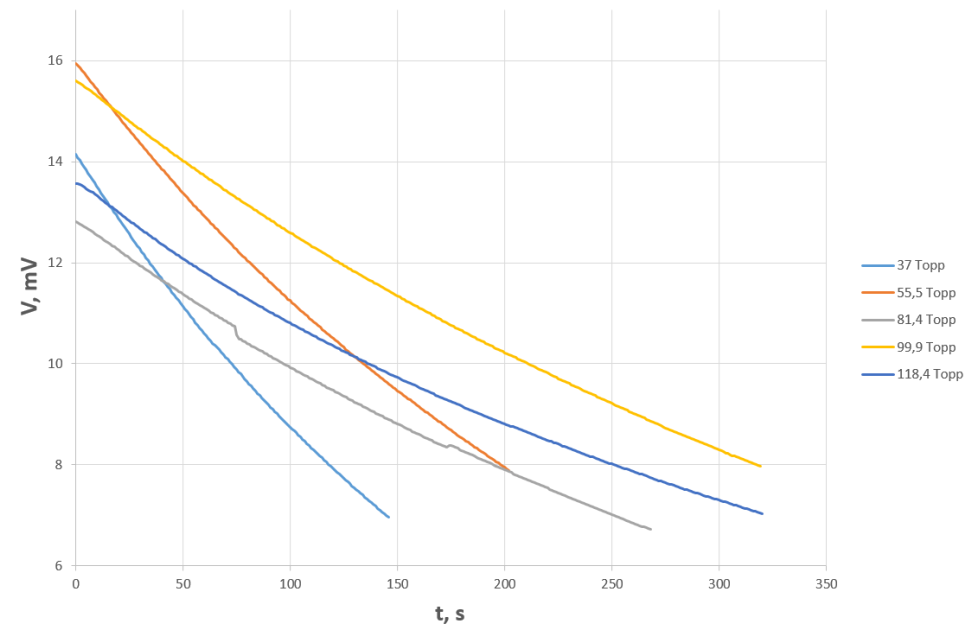
\includegraphics[width=0.8\linewidth]{data 2_2_1.png}
    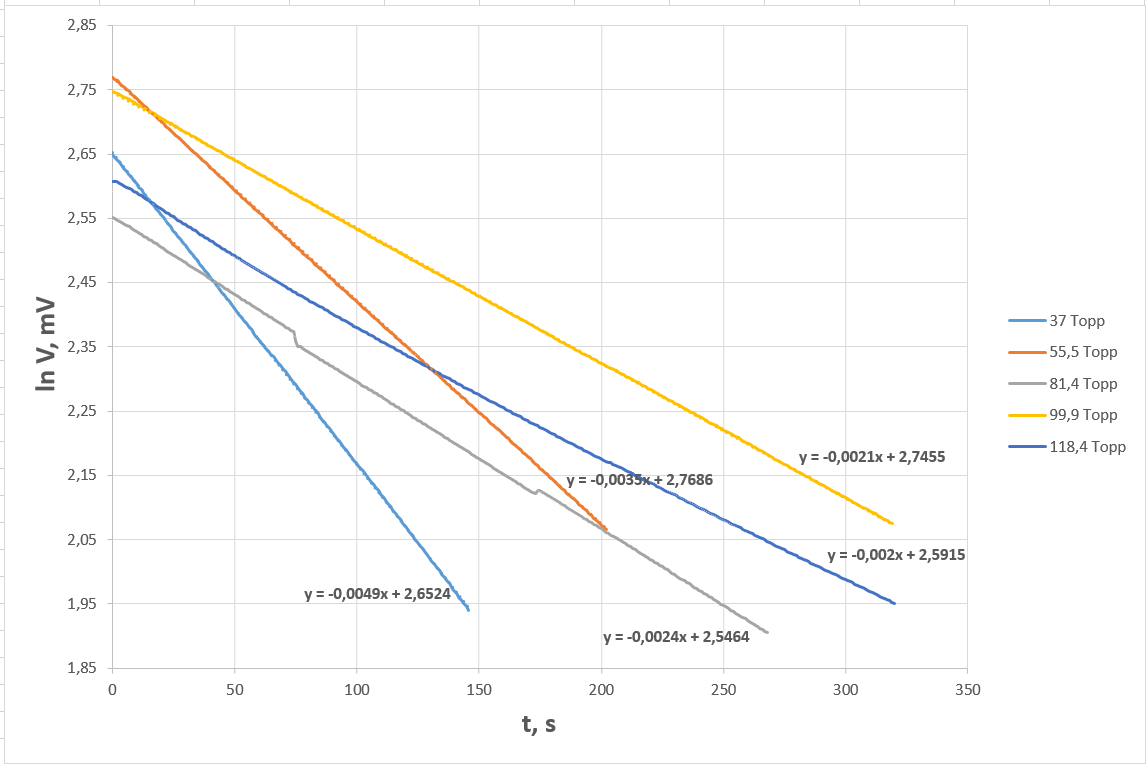
\includegraphics[width=0.8\linewidth]{lines 2.2.1.png}
    \caption{Получившиеся графики}
\end{figure}
\newpage
Итого, получилисть следующие значение величины \(1/\tau\):
\begin{table}[h]
    \centering
     \begin{tabular}{|c|c|c|}
    \hline
         \(P_{раб}\), Торр & \(\tau\), с & \(\Delta \tau\), с \\
    \hline
         37,0  & 204,08 & 0,14 \\
         55,5  & 285,71 & 0,32 \\
         81,4  & 416,67 & 0,46 \\
         99,9  & 476,19 & 0,87 \\
         118,4 & 500,01 & 0,93 \\
    \hline
    \end{tabular}
\end{table}

Таким образом, посчитаем коэффициенты \(D\) по формуле \(D = \frac{V_1 V_2}{V_1 + V_2}\frac{l}{S\tau}\). Получится:
\begin{table}[h]
    \centering
    \begin{tabular}{|c|c|c|}
    \hline
         \(P_{раб}\), Торр & D, \(см^2c^{-2}\) & \(\Delta\)D, \(см^2c^{-2}\) \\
    \hline
         37,0  & 10.06 & 0,23\\
         55,5  & 7.19  & 0,16 \\
         81,4  & 4.9   & 0,11\\
         99,9  & 4.31  & 0,10\\
         118,4 & 4.1   & 0,09\\
    \hline
    \end{tabular}
\end{table}
\\
\\
Построим график \(D(1/P)\):
\begin{figure}[h]
    \centering
    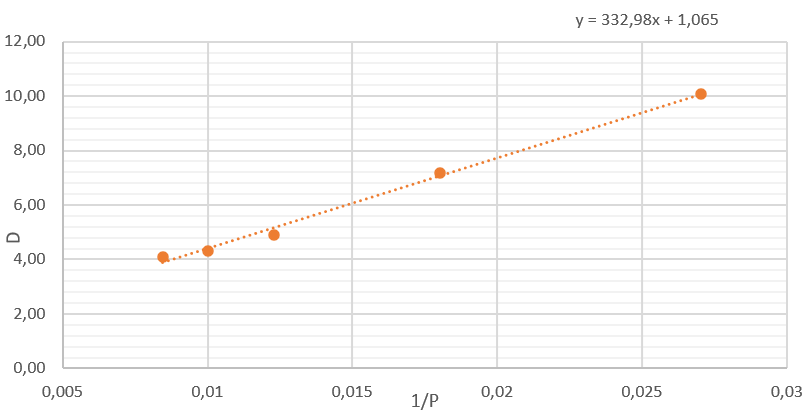
\includegraphics[width=0.8\linewidth]{DP.png}
\end{figure}

Как видно, точки легли на прямую (с точностью до какого-то значения). Значит, коэффициент взаимной диффузии линейно зависит от величины, обратной давлению. Таким образом найдем $D(P_0) = 0,44 \pm 0.05 см^2c^{-1}$
\\
\\

Теперь найдем длину свободного пробега и эффективное сечение столкновений по формулам:
\[\lambda = 3D\sqrt{\frac{\pi \mu}{8RT}} = 104,8 \pm 6,3 нм\]
\[\sigma = \frac{1}{n_0\lambda} = 3,95 \cdot 10^{-19} м^2\]
\section{Заключение:} 
Мы провели ряд экспериментов, в результате которых получили коэффиценты взаимной диффузии при различных давлениях. Также мы получили этот коэффициент для атмосферного давления, он немного не сошелся с табличными данными. Также мы убедились, что коэффициент линейно зависит от величины, обратной давлению.

\end{document}
